\documentclass[10pt]{article}
\usepackage{amsmath, amssymb}
\usepackage[ngerman]{babel}
\usepackage[margin=1in]{geometry}
\usepackage{enumitem}
\usepackage{graphicx}
\usepackage{float}

\newcommand{\NN}{\mathcal{N}}
\newcommand{\R}{\mathcal{R}}
\newcommand{\BB}{\mathcal{B}}
\newcommand{\KK}{\mathcal{K}}


\begin{document}
\section{Order Packaging Optimization}

%%════════════════════════════════════════════════
\subsection{Einleitung}
\label{sec:einleitung}
%%════════════════════════════════════════════════

Die effiziente Verpackung von Produkten in Versandkartons ist ein
zentrales Optimierungsproblem der modernen Logistik.
Insbesondere im E-Commerce werden t\"aglich Millionen von Bestellungen kommissioniert und versendet,
wobei ungeeignete Kartonwahl zu unn\"otigem Leerraum, h\"oheren
Versandkosten und erh\"ohtem Materialverbrauch f\"uhrt.
Dar\"uber hinaus entstehen erhebliche Transportsch\"aden, wenn schwere
Produkte auf empfindlichen Artikeln platziert werden oder fragile Waren
ohne ausreichende Stabilit\"at im Karton verrutschen --- Verluste, die
direkt zu Retouren und Reklamationen f\"uhren.
Eine automatisierte Packplanung kann diese Kosten
senken und gleichzeitig sicherstellen, dass Produkte
transportsicher und besch\"adigungsfrei beim Kunden ankommen.
Der folgende Abschnitt beschreibt eine mehrstufige MILP-basierte Pipeline,
die genau dieses Problem l\"ost: Sie weist Produkte geeigneten Kartons zu
und optimiert deren r\"aumliche Anordnung unter physikalischen
Qualit\"atskriterien.

%%════════════════════════════════════════════════
\subsection{Problemdefinition}
\label{sec:problem}
%%════════════════════════════════════════════════

Gegeben ist eine \emph{Transaktion}: eine Menge von $n$ Produkten
$\{p_1, \dots, p_n\}$, wobei jedes Produkt $p_i$ seine physischen
Dimensionen $(l_i, w_i, d_i)$ (L\"ange, Breite, Tiefe in cm) sowie sein
Gewicht $m_i$ (in kg) hat.
Gesucht ist eine Aufteilung der Produkte auf eine minimale Anzahl von
Versandkartons sowie, f\"ur jeden Karton, eine zul\"assige und qualitativ
hochwertige r\"aumliche Anordnung der ihm zugewiesenen Produkte.

\paragraph{Transaktionstrennung.}
Die einfachste denkbare L\"osung (alle Produkte in einen einzigen,
hinreichend gro\ss en Karton zu legen) ist in der Praxis nicht
umsetzbar.
Logistische und ergonomische Vorgaben begrenzen das Gesamtgewicht und
die Produktanzahl pro Karton.
Zus\"atzlich d\"urfen Produkte mit stark unterschiedlichen Gewichten
nicht gemeinsam verpackt werden, da das schwerere Produkt das
leichtere besch\"adigen k\"onnte (wir vermuten, dass das Gewicht mit der Fragilit\"at korreliert).
Schlie\ss lich sind \"uberm\"a\ss ig gro\ss e Leerr\"aume unerw\"unscht,
da sie die Stabilit\"at der Packung verringern und Versandkosten
erh\"ohen.
Diese Randbedingungen machen eine explizite \emph{Transaktionstrennung}
notwendig (Abschnitt~\ref{sec:s0}), die mittels
Bin-Packing-MILP die Produkte in Teiltransaktionen zerlegt, von denen
jede genau einem Karton entspricht.

\paragraph{Boxauswahl.}
Es stehen vordefinierte Kartontypen zur Verfügung; das Boxauswahl-MILP (Abschnitt~\ref{sec:boxauswahl}) weist jeder Teiltransaktion einen passenden Typ zu und stellt sicher, dass die Produkte dieser Teiltransaktion in dem Kartontyp gepackt werden können.

\paragraph{Packqualit\"at.}
Eine zul\"assige Packung (d.\,h.\ eine Anordnung ohne gegenseitige
\"Uberlappungen, bei der alle Produkte vollst\"andig im Karton liegen) 
stellt jedoch nur eine notwendige, keine hinreichende Bedingung dar.
Dar\"uber hinaus soll die Packung physikalisch stabil und transportsicher
sein: Schwere Produkte sind nach unten zu legen, leichte nach oben;
fl\"achige Produkte sollen eine breite, stabile Basis bilden, w\"ahrend
kleinere Produkte dar\"uber angeordnet werden; Produkte sollen vorzugsweise
auf ihrer gr\"o\ss ten Fl\"ache aufliegen; und leichte, potenziell
empfindliche Produkte d\"urfen nicht von schwereren belastet werden.
Diese Qualit\"atskriterien werden in Packqualit\"at (Abschnitt~\ref{sec:s2})
als gewichtete Terme eines nicht-konvexen MIQP formuliert und optimiert.

\paragraph{Laufzeitanforderungen.}
Das beschriebene Optimierungsproblem ist NP-schwer; exakte L\"osungen sind
im Allgemeinen nur f\"ur kleine Instanzen in vertretbarer Zeit erreichbar.
Im Kontext der Lagerlogistik unterliegt die Berechnung jedoch einer harten
Zeitschranke: Die Packl\"osung muss w\"ahrend der laufenden Transaktionsbearbeitung
bestimmt werden, sodass dem Solver insgesamt h\"ochstens wenige Sekunden  zur
Verf\"ugung stehen.
Diese Anforderung beeinflusst die Modellwahl unmittelbar. Komplexe
Formulierungen mit vielen bin\"aren Variablen oder nichtlinearen Termen
sind nur dann tragbar, wenn sie in der Praxis relevante Instanzen
zuverl\"assig innerhalb dieses Zeitfensters l\"osen.
Die mehrstufige Pipeline tr\"agt diesem Umstand Rechnung, indem sie die
Gesamtkomplexität auf spezialisierte, sequenziell ausgef\"uhrte Teilmodelle verteilt.

%%════════════════════════════════════════════════
\subsection{Packing Pipeline}
\label{sec:pipe2}
%%════════════════════════════════════════════════


\begin{center}
Boxtypen + Transaktion \\[4pt]
$\downarrow$ \\[4pt]
Transaktionstrennung-MILP \\[4pt]
$\downarrow$ \\[4pt]
Boxauswahl-MILP \\[4pt]
$\downarrow$ \\[4pt]
3D-Packqualit\"at-MIQP \\[4pt]
$\downarrow$ \\[4pt]
Gepackte Produkte
\end{center}

\paragraph{Transaktionstrennung-MILP}
Bevor Produkte in Kartons gepackt werden, muss entschieden werden,
welche Produkte \"uberhaupt gemeinsam verschickt werden sollen.
Gro\ss e Transaktionen oder Transaktionen mit sehr unterschiedlichen
Gewichten k\"onnen aus logistischer Sicht nicht sinnvoll in einem einzigen Karton zusammengefasst werden.
Transaktionstrennung l\"ost deshalb ein MILP Bin-Packing, das die Transaktion in
m\"oglichst wenige Teiltransaktionen zerlegt.
Jede Teiltransaktion muss das Gewichtskapazit\"atslimit einhalten, und Produktpaare mit stark
unterschiedlichem Gewicht werden durch Inkompatibilit\"atsbedingungen
in separate Bins gezwungen. Dies soll sp\"atere Besch\"adigungen durch
schwere auf leichten Produkten verhindern.
Dieses Teilproblem entspricht dem klassischen \emph{Bin-Packing-Problem}
(1D, Gewichtskapazit\"at), das NP-schwer ist.
\emph{Formulierung in Abschnitt~\ref{sec:s0}.}

\paragraph{Boxauswahl-MILP.}
F\"ur jede Teiltransaktion muss ein passender Karton aus dem vorgegebenen
Sortiment gew\"ahlt werden und gleichzeitig muss
gepr\"uft werden, ob die Produkte \"uberhaupt r\"aumlich in diesen
Karton passen.
Da Boxwahl und Packbarkeit voneinander abh\"angen, werden beide
Entscheidungen in einem einzigen MILP gemeinsam gel\"ost.
Das Modell weist Produkte Bins zu, w\"ahlt pro Bin einen Boxtyp und
erzwingt dabei vollst\"andige 3D-\"Uberlappungsfreiheit aller
Produkte.
Zus\"atzliche Bedingungen stellen sicher, dass kein Karton \"uberladen
wird (ein Limit für die Anzahl von Produkten in einem Karton) und der Leerraum einen Mindestf\"ullgrad von $50\%$ nicht unterschreitet.
Die Zielfunktion minimiert die Anzahl ben\"otigter Kartons; nicht
zuordenbare Produkte werden mit einer Strafgewichtung belegt,
sodass das Modell auch in unl\"osbaren Teilinstanzen eine
brauchbare L\"osung liefert.
Dieses Teilproblem entspricht dem \emph{3D Bin Packing Problem (3D-BPP)},
das stark NP-schwer ist.
\emph{Formulierung in Abschnitt~\ref{sec:boxauswahl}.}

% \paragraph{Bounding-Box-Minimierung-MILP}
% Neben dieser Pipeline existiert eine alternative Pipeline zur
% \emph{freien Boxoptimierung}, bei der keine Boxtypen vorgegeben werden.
% Dort \"ubernimmt Bounding-Box-Minimierung (Abschnitt~\ref{sec:s1})
% die Rolle der Boxbestimmung: Sie liefert eine geometrisch optimale Box
% direkt aus den Produktabmessungen sowie eine initiale Packung als Warmstart
% f\"ur Packqualit\"atsoptimierung.
% Die freie Pipeline ben\"otigt ausschlie\ss{}lich die Produktliste als Eingabe
% und kennt keinen Einzelversandfall, da die Box stets an die Produkte
% angepasst wird.
% Dieses Teilproblem entspricht dem \emph{3D Strip Packing Problem (3D-SPP)},
% das ebenfalls stark NP-schwer ist.

\paragraph{3D-Packqualität-MIQP}
Das Boxauswahl-MILP legt fest, \emph{welche} Produkte in \emph{welchen}
Karton geh\"oren und liefert bereits eine geometrisch g\"ultige
Packung. Diese ist jedoch nicht notwendigerweise physikalisch
sinnvoll.
Packqualit\"atsoptimierung verbessert deshalb die Anordnung durch ein nicht-konvexes
MIQP, wobei die Ausgabe von
Boxauswahl-MILP als Warmstart dient und die L\"osungszeit erheblich
verk\"urzt.
Die Zielfunktion ist eine gewichtete Summe aus f\"unf Termen:
\textbf{Flachheit} beg\"unstigt gro\ss e Auflagefl\"achen;
\textbf{Pyramide} dr\"angt breitere Produkte nach unten;
\textbf{Schwerkraft} zieht schwere Produkte tief in den Karton;
\textbf{Fragilit\"at} bestraft Anordnungen, in denen schwere Produkte
auf leichten liegen; und die quadratische
Dieses Teilproblem entspricht dem \emph{Container Loading Problem (CLP)}
mit physikalischen Stabilit\"ats- und Fragilit\"atsbedingungen.
\emph{Formulierung in Abschnitt~\ref{sec:s2}.}

%%════════════════════════════════════════════════
\subsection{Transaktionstrennung}
\label{sec:s0}
%%════════════════════════════════════════════════

Gegeben: $n$ Produkte einer Transaktion.
MILP Bin-Packing zur Aufteilung in Teiltransaktionen mit Gewichts-,
Kapazit\"ats- und Kompatibilit\"atsbeschr\"ankungen.

\paragraph{Mengen}

\begin{alignat*}{2}
\NN &= \{1, \dots, n\}
  &\qquad& \text{Menge der Produkte} \\
\BB &= \{1, \dots, n\}
  && \text{Menge der Teiltransaktionen (obere Schranke)} \\
\end{alignat*}

\paragraph{Eingabedaten und Modellkonstanten}

\begin{alignat*}{2}
m_i &\in \mathbb{R}_{>0}
  &\qquad& \text{Gewicht von Produkt $i$} \\
W_{\max} &= 10{,}0
  && \text{max.\ Gewicht pro Bin} \\
R &= 5{,}0
  && \text{Gewichtsverh\"altnis f\"ur Inkompatibilit\"at} \\
H &= 0{,}5
  && \text{Schwellenwert f\"ur ,,schwer''}
\end{alignat*}

\paragraph{Abgeleitete Gr\"o\ss en}

Inkompatible Paare: Produkte $i, j$ d\"urfen nicht im selben Bin liegen.
\begin{alignat*}{2}
\mathcal{I} &= \bigl\{\, (i,j) \mid \;
  \max(m_i, m_j) \geq H,\;
  \tfrac{\max(m_i, m_j)}{\min(m_i, m_j)} \geq R
  \,\bigr\}
  &\qquad& \text{inkompatible Paare} \\
\end{alignat*}

\paragraph{Entscheidungsvariablen}

\begin{alignat*}{2}
x_{ib} &\in \{0,1\},\; i \in \NN,\; b \in \BB
  &\qquad& \text{Produkt $i$ ist Bin $b$ zugeordnet} \\
y_b &\in \{0,1\},\; b \in \BB
  && \text{Bin $b$ wird verwendet} \\
\end{alignat*}

\paragraph{Nebenbedingungen}

Jedes Produkt genau einem Bin zugeordnet.
\begin{alignat*}{2}
\sum_{b \in \BB} x_{ib} &= 1
  &\qquad& \forall\, i \in \NN
\end{alignat*}

Gesamtgewicht pro Bin durch $W_{\max}$ beschr\"ankt; koppelt $x$ an $y$. Produkte mit $m_i > W_{\max}$ werden als Einzeltransaktionen abgespalten.
\begin{alignat*}{2}
\sum_{i \in \NN} m_i\, x_{ib} &\leq W_{\max}\, y_b
  &\qquad& \forall\, b \in \BB
\end{alignat*}

Inkompatible Paare d\"urfen nicht im selben Bin liegen.
\begin{alignat*}{2}
x_{ib} + x_{jb} &\leq 1
  &\qquad& \forall\, (i,j) \in \mathcal{I},\; \forall\, b \in \BB
\end{alignat*}

Bins werden in aufsteigender Reihenfolge belegt.
\begin{alignat*}{2}
y_b &\leq y_{b-1}
  &\qquad& \forall\, b \in \BB,\; b \geq 2
\end{alignat*}

\paragraph{Zielfunktion}

\begin{equation*}
\min \quad \sum_{b \in \BB} y_b
\end{equation*}

Minimiert die Anzahl verwendeter Bins (= Teiltransaktionen).

%%════════════════════════════════════════════════
\subsection{Boxauswahl}
\label{sec:boxauswahl}
%%════════════════════════════════════════════════

Gegeben: $n$ Produkte, $K$ Boxtypen (jeweils unbegrenzt verf\"ugbar).
MILP zur Zuordnung von Produkten zu Bins mit vollst\"andiger
3D-\"Uberlappungsfreiheit und Boxtypauswahl.

\paragraph{Mengen}

\begin{alignat*}{2}
\NN &= \{1, \dots, n\}
  &\qquad& \text{Menge der Produkte} \\
\KK &= \{1, \dots, K\}
  && \text{Menge der Boxtypen} \\
\BB &= \{1, \dots, n\}
  && \text{Menge der Bins (obere Schranke)} \\
\R &= \{1, \dots, 6\}
  && \text{Menge der Rotationen} \\
\end{alignat*}

\paragraph{Eingabedaten und abgeleitete Gr\"o\ss en}

\begin{alignat*}{2}
\sigma_k &= (\sigma_k^1, \sigma_k^2, \sigma_k^3),\; k \in \R
  &\qquad& \text{$k$-te Permutation von $\{1,2,3\}$} \\
\mathbf{p}_i &= (p_i^1, p_i^2, p_i^3)
  && \text{L\"ange, Breite, Tiefe von Produkt $i$} \\
v_i &= p_i^1 \cdot p_i^2 \cdot p_i^3
  && \text{Volumen von Produkt $i$} \\
(B_k^x, B_k^y, B_k^z) &,\; k \in \KK
  && \text{Dimensionen von Boxtyp $k$} \\
V_k &= B_k^x \cdot B_k^y \cdot B_k^z
  && \text{Volumen von Boxtyp $k$} \\
\end{alignat*}

\paragraph{Modellkonstanten}

\begin{alignat*}{2}
M_x &= \max_k B_k^x
  &\qquad& \text{Big-M-Werte} \\
M_y &= \max_k B_k^y && \\
M_z &= \max_k B_k^z && \\
P &= 7
  && \text{max.\ Produkte pro Bin} \\
\phi &= 0{,}5
  && \text{max.\ Freivolumenanteil} \\
\lambda &= 100
  && \text{Strafe f\"ur nicht zugeordnete Produkte} \\
\end{alignat*}

\paragraph{Entscheidungsvariablen}
\label{sec:s2:vars}

\begin{alignat*}{2}
x_i, y_i, z_i &\geq 0
  &\qquad& \text{Ursprungskoordinaten von Produkt $i$} \\
\Delta x_i, \Delta y_i, \Delta z_i &\in \mathbb{Z}
  && \text{effektive Dimensionen nach Rotation} \\
r_{ik} &\in \{0,1\},\; k \in \R
  && \text{Rotationsauswahl}
\end{alignat*}

Produkt $i$ belegt $[x_i, x_i{+}\Delta x_i] \times [y_i, y_i{+}\Delta y_i] \times [z_i, z_i{+}\Delta z_i]$.
Obergrenzen hier: $M_x, M_y, M_z$ statt fester Boxabmessungen.

\begin{alignat*}{2}
a_{ib} &\in \{0,1\},\; i \in \NN,\; b \in \BB
  &\qquad& \text{Produkt $i$ ist Bin $b$ zugeordnet} \\
y_b &\in \{0,1\},\; b \in \BB
  && \text{Bin $b$ wird verwendet} \\
t_{bk} &\in \{0,1\},\; b \in \BB,\; k \in \KK
  && \text{Bin $b$ verwendet Boxtyp $k$}
\end{alignat*}

\begin{alignat*}{2}
\sigma_{ij} &\in \{0,1\}\;
  &\qquad& \text{$i$ und $j$ im selben Bin} \\
s_{ij}^d &\in \{0,1\},\; d \in \{1,\dots,6\}\;
  && \text{Separationsrichtung}
\end{alignat*}

\paragraph{Nebenbedingungen}

\label{sec:s2:rotation}
Genau eine der sechs Rotationen pro Produkt.
Die sechs Rotationen entsprechen allen Permutationen der drei Dimensionen
$(w, l, d)$ auf die Achsen $(x, y, z)$.
Drei Rotationen (um die Hauptachsen) w\"urden nicht alle m\"oglichen
Zuordnungen abdecken --- z.\,B.\ kann eine reine 90°-Drehung nicht
$(w \to z,\; l \to x,\; d \to y)$ erzeugen.
\begin{alignat*}{2}
\sum_{k \in \R} r_{ik} &= 1
  &\qquad& \forall\, i \in \NN
\end{alignat*}

Effektive Dimensionen gem\"a\ss{} gew\"ahlter Rotation.
\begin{alignat*}{2}
\Delta x_i &= \textstyle\sum_k r_{ik}\, p_i^{\sigma_k^1}
  &\qquad& \forall\, i \in \NN \\
\Delta y_i &= \textstyle\sum_k r_{ik}\, p_i^{\sigma_k^2}
  && \forall\, i \in \NN \\
\Delta z_i &= \textstyle\sum_k r_{ik}\, p_i^{\sigma_k^3}
  && \forall\, i \in \NN
\end{alignat*}

Jedes Produkt h\"ochstens einem aktiven Bin zugeordnet.
\begin{alignat*}{2}
\sum_{b \in \BB} a_{ib} &\leq 1
  &\qquad& \forall\, i \in \NN \\
a_{ib} &\leq y_b
  && \forall\, i \in \NN,\; b \in \BB
\end{alignat*}

Jeder aktive Bin erh\"alt genau einen Boxtyp.
\begin{alignat*}{2}
\sum_{k \in \KK} t_{bk} &= y_b
  &\qquad& \forall\, b \in \BB
\end{alignat*}

Produkte m\"ussen in die Dimensionen ihres Bins passen.
\begin{alignat*}{2}
x_i + \Delta x_i &\leq \textstyle\sum_k t_{bk}\, B_k^x + M_x(1 - a_{ib})
  &\qquad& \forall\, i,\, b \\
y_i + \Delta y_i &\leq \textstyle\sum_k t_{bk}\, B_k^y + M_y(1 - a_{ib})
  && \forall\, i,\, b \\
z_i + \Delta z_i &\leq \textstyle\sum_k t_{bk}\, B_k^z + M_z(1 - a_{ib})
  && \forall\, i,\, b
\end{alignat*}

Gleicher-Bin-Verkn\"upfung.
\begin{alignat*}{2}
\sigma_{ij} &\geq a_{ib} + a_{jb} - 1
  &\qquad& \forall\, i < j,\; \forall\, b \in \BB
\end{alignat*}

Produkte im selben Bin m\"ussen entlang mind.\ einer Achse getrennt sein.
Big-M wird bei $\sigma_{ij} = 0$ zus\"atzlich relaxiert.
\begin{alignat*}{2}
\textstyle\sum_{d=1}^{6} s_{ij}^d &\geq \sigma_{ij}
  &\qquad& \\[4pt]
x_i + \Delta x_i &\leq x_j + M_x(1 - s_{ij}^1) + M_x(1 - \sigma_{ij}) \\
x_j + \Delta x_j &\leq x_i + M_x(1 - s_{ij}^2) + M_x(1 - \sigma_{ij}) \\
y_i + \Delta y_i &\leq y_j + M_y(1 - s_{ij}^3) + M_y(1 - \sigma_{ij}) \\
y_j + \Delta y_j &\leq y_i + M_y(1 - s_{ij}^4) + M_y(1 - \sigma_{ij}) \\
z_i + \Delta z_i &\leq z_j + M_z(1 - s_{ij}^5) + M_z(1 - \sigma_{ij}) \\
z_j + \Delta z_j &\leq z_i + M_z(1 - s_{ij}^6) + M_z(1 - \sigma_{ij}) \\
\end{alignat*}

Max.\ $P$ Produkte pro Bin.
\begin{alignat*}{2}
\sum_{i \in \NN} a_{ib} &\leq P
  &\qquad& \forall\, b \in \BB
\end{alignat*}

Bins in aufsteigender Reihenfolge belegt.
\begin{alignat*}{2}
y_b &\geq y_{b+1}
  &\qquad& \forall\, b \in \{1, \dots, |\BB|-1\}
\end{alignat*}

Produkte m\"ussen mind.\ $(1 - \phi)$ des Boxvolumens f\"ullen.
\begin{alignat*}{2}
\sum_{i \in \NN} v_i\, a_{ib} &\geq (1 - \phi) \sum_{k \in \KK} t_{bk}\, V_k
  &\qquad& \forall\, b \in \BB
\end{alignat*}

\paragraph{Zielfunktion}

\begin{equation*}
\min \quad
  \sum_{b \in \BB} y_b
  \;+\;
  \lambda \sum_{i \in \NN} \Bigl(1 - \sum_{b \in \BB} a_{ib}\Bigr)
\end{equation*}

Minimiert Bin-Anzahl mit hoher Strafe f\"ur nicht zugeordnete Produkte.

% %%════════════════════════════════════════════════
% \subsection{Bounding-Box-Minimierung}
% \label{sec:s1}
% %%════════════════════════════════════════════════

% Gegeben: $n$ Produkte, initiale Boxschranke $(B_x, B_y, B_z)$.
% MILP zur Minimierung der Bounding-Box-Dimensionen;

% \paragraph{Mengen und Parameter}

% \begin{alignat*}{2}
% \NN &= \{1, \dots, n\}
%   &\qquad& \text{Menge der Produkte} \\
% \R &= \{1, \dots, 6\}
%   && \text{Menge der Rotationen} \\
% \mathbf{p}_i &= (p_i^1, p_i^2, p_i^3)
%   &\qquad& \text{L\"ange, Breite, Tiefe von Produkt $i$} \\
% V_{\mathrm{prod}} &= \textstyle\sum_{i \in \NN} p_i^1 \cdot p_i^2 \cdot p_i^3
%   &\qquad& \text{Gesamtvolumen der Produkte} \\
% \alpha &= 2
%   && \text{max.\ zul\"assiges Boxvolumenverh\"altnis}
% \end{alignat*}

% \paragraph{Entscheidungsvariablen}

% Positions- und Dimensionsvariablen $(x_i, y_i, z_i, \Delta x_i, \Delta y_i, \Delta z_i)$
% wie in Abschnitt~\ref{sec:s2:vars}.

% \begin{alignat*}{2}
% X_{\max}, Y_{\max}, Z_{\max} &\in \mathbb{Z}_{\geq 0}
%   &\qquad& \text{Packungsausdehnung (ganzzahlig)} \\
% A_{xy} &\geq 0
%   &\qquad& \text{Fl\"ache der XY-Grundseite}
% \end{alignat*}

% \paragraph{Nebenbedingungen}

% Rotation und Dimensionsverkn\"upfung wie in~\ref{sec:s2:rotation}.
% \"Uberlappungsfreiheit wie in~\ref{sec:s2:nooverlap}.
% Bounding-Box wie in~\ref{sec:s2:bbox}, hier mit $\mathbb{Z}$-Variablen.

% Produkte nach Positionssumme geordnet.
% \begin{alignat*}{2}
% x_i + y_i + z_i &\geq x_{i-1} + y_{i-1} + z_{i-1}
%   &\qquad& \forall\, i \in \{2, \dots, n\}
% \end{alignat*}
% Diese Symmetriebrechung verhindert gespiegelte L\"osungen:
% ohne sie k\"onnte der Solver zwei \"aquivalente Packungen finden,
% die sich nur in der Reihenfolge der Produkte unterscheiden.


% Boxvolumen darf das Produktvolumen h\"ochstens um Faktor $\alpha$ \"ubersteigen.
% \begin{alignat*}{2}
% A_{xy} &= X_{\max} \cdot Y_{\max}
%   &\qquad& \text{(quadratisch)} \\
% A_{xy} \cdot Z_{\max} &\leq \alpha \cdot A_{\mathrm{prod}}
%   && \text{(kubisch $\Rightarrow$ \texttt{NonConvex=2})}
% \end{alignat*}
% Die Hilfsvariable $A_{xy}$ linearisiert das Produkt $X_{\max} \cdot Y_{\max}$
% in einer separaten quadratischen Nebenbedingung, sodass die kubische
% Volumenrestriktion als bilineare Ungleichung $A_{xy} \cdot Z_{\max} \leq \ldots$
% formuliert werden kann.

% \paragraph{Zielfunktion}

% \begin{equation}
% \min \quad X_{\max} + Y_{\max} + Z_{\max}
% \end{equation}

% Minimiert die Summe der Bounding-Box-Dimensionen.
% Die Summenminimierung bevorzugt w\"urfel\"ahnliche Bounding-Boxes,
% da bei gleichem Volumen der W\"urfel die kleinste Dimensionssumme besitzt.
% Eine reine Volumenminimierung w\"urde dagegen flache Packungen erzeugen,
% was f\"ur den nachfolgenden Packqualit\"atsschritt ung\"unstig ist.

%%════════════════════════════════════════════════
\subsection{3D-Packqualit\"at MIQP}
\label{sec:s2}
%%════════════════════════════════════════════════

Gegeben: $n$ Produkte, Zielbox $(B_x, B_y, B_z)$.
Nicht-konvexes MIQP mit Warmstart aus Boxauswahl-MILP.

\paragraph{Mengen}
\begin{alignat*}{2}
\NN &= \{1, \dots, n\}
  &\qquad& \text{Menge der Produkte} \\
\R &= \{1, \dots, 6\}
  && \text{Menge der Rotationen}
\end{alignat*}

\paragraph{Eingabedaten und abgeleitete Gr\"o\ss en}
\begin{alignat*}{2}
\sigma_k &= (\sigma_k^1, \sigma_k^2, \sigma_k^3),\; k \in \R
  && \text{$k$-te Permutation von $\{1,2,3\}$} \\
\mathbf{p}_i &= (p_i^1, p_i^2, p_i^3)
  &\qquad& \text{L\"ange, Breite, Tiefe von Produkt $i$} \\
m_i &\in \mathbb{R}_{>0}
  && \text{Gewicht von Produkt $i$} \\
\delta_i^{\min} &= \min(p_i^1, p_i^2, p_i^3)
  &\qquad& \text{kleinste Dimension} \\
\mathcal{A}_i &= \bigl\{ p_i^a p_i^b \mid (a,b) \in \{(1,2),(1,3),(2,3)\} \bigr\}
  && \text{drei Seitenfl\"achen} \\
F_i^{\min} &= \min \mathcal{A}_i
  && \text{kleinste Seitenfl\"ache} \\
F_i^{\max} &= \max \mathcal{A}_i
  && \text{gr\"o\ss te Seitenfl\"ache} \\
\rho_i &= F_i^{\max} / F_i^{\min}
  && \text{Fl\"achenverh\"altnis} \\
m_{\min} &= \min_\NN m_i, \quad m_{\max} = \max_\NN m_i
  && \text{Gewichtsschranken} \\
\tilde{m}_i &= (m_i^2 - m_{\min}^2) / (m_{\max}^2 - m_{\min}^2)
  && \text{norm.\ Gewicht (quadr.\ Skalierung)} \\
F_{\mathrm{abs}}^{\min} &= \min_i F_i^{\min}
  && \text{globale min.\ Fl\"ache} \\
F_{\mathrm{abs}}^{\max} &= \max_i F_i^{\max}
  && \text{globale max.\ Fl\"ache}
\end{alignat*}

\paragraph{Zielfunktionsgewichte}
\begin{alignat*}{2}
w_{\mathrm{flat}} &= 10{,}0
  &\qquad& \text{Flachheit --- bestraft kleine Auflagefl\"achen, skal.\ mit $\rho_i$} \\
w_{\mathrm{pyr}} &= 7{,}0
  && \text{Pyramide --- breite Basis unten, schmale Spitze oben} \\
w_{\mathrm{grav}} &= 5{,}0
  && \text{Schwerkraft --- schwere Produkte nach unten} \\
w_{\mathrm{frag}} &= 10{,}0
  && \text{Fragilit\"at --- bestraft Schwer-auf-Leicht ($m_j/m_i$)} \\
\tau &= 0
  && \text{W\"urfel\"ahnlichkeitsschwelle (Rotationspruning)}
\end{alignat*}

Warmstart aus Boxauswahl-MILP.
W\"urfel\"ahnliche Produkte ($\tau = 0$) k\"onnen
\"aquivalente Rotationen fixieren.
Pyramidenterm $\Rightarrow$ nicht-konvexes MIQP.

\paragraph{Entscheidungsvariablen}

Positions-, Dimensions- und Rotationsvariablen wie in Abschnitt~\ref{sec:s2:vars}.

\begin{alignat*}{2}
s_{ij}^d &\in \{0,1\},\; d \in \{1,\dots,6\},\; i < j
  &\qquad& \text{Separationsrichtung} \\
a_{ji} &\in \{0,1\},\; i \neq j
  && \text{$j$ liegt \"uber $i$} \\
X_{\max}, Y_{\max}, Z_{\max} &\geq 0
  && \text{Packungsausdehnung} \\
f_{\min}, f_{\max} &\in [F_{\mathrm{abs}}^{\min}, F_{\mathrm{abs}}^{\max}]
  && \text{min/max Grundfl\"ache} \\
\hat{f}_i &\in [0, 1]
  && \text{global normierte Grundfl\"ache}
\end{alignat*}

\paragraph{Nebenbedingungen}

Rotation und Dimensionsverkn\"upfung wie in Abschnitt~\ref{sec:s2:rotation}.

\label{sec:s2:nooverlap}
Jedes Paar entlang mind.\ einer Halbachse getrennt (Big-M, achsenspez.).
F\"ur jedes Produktpaar $(i,j)$ wird gefordert, dass mindestens eine
der sechs Halbachsenrichtungen ($x^+, x^-, y^+, y^-, z^+, z^-$) als
Trennrichtung aktiv ist.
Die Big-M-Werte sind achsenspezifisch ($B_x, B_y, B_z$ statt eines
globalen $M$), um die LP-Relaxation zu versch\"arfen.
\begin{alignat*}{2}
\textstyle\sum_{d=1}^{6} s_{ij}^d &\geq 1
  &\qquad& \forall\, i < j \\[4pt]
x_i + \Delta x_i &\leq x_j + B_x(1 - s_{ij}^1)
  && \forall\, i < j \\
x_j + \Delta x_j &\leq x_i + B_x(1 - s_{ij}^2)
  && \forall\, i < j \\
y_i + \Delta y_i &\leq y_j + B_y(1 - s_{ij}^3)
  && \forall\, i < j \\
y_j + \Delta y_j &\leq y_i + B_y(1 - s_{ij}^4)
  && \forall\, i < j \\
z_i + \Delta z_i &\leq z_j + B_z(1 - s_{ij}^5)
  && \forall\, i < j \\
z_j + \Delta z_j &\leq z_i + B_z(1 - s_{ij}^6)
  && \forall\, i < j
\end{alignat*}

% \label{sec:s2:bbox}
% Obere Schranke der Packungsausdehnung.
% Die Bounding-Box-Variablen werden nicht auf $(B_x, B_y, B_z)$ fixiert,
% da das Modell eine kontrollierte \"Uberschreitung der Zielbox erlaubt
% (siehe \"Uberschreitungsvariablen $e_x, e_y, e_z$ unten).
% \begin{alignat*}{2}
% X_{\max} &\geq x_i + \Delta x_i
%   &\qquad& \forall\, i \in \NN \\
% Y_{\max} &\geq y_i + \Delta y_i
%   && \forall\, i \in \NN \\
% Z_{\max} &\geq z_i + \Delta z_i
%   && \forall\, i \in \NN
% \end{alignat*}

% Wie weit die Packung die Zielbox \"uberschreitet.
% Die \"Uberschreitungsvariablen $e_x, e_y, e_z \geq 0$ messen, um wie viel
% die Packungsausdehnung die Zielbox \"ubersteigt.
% Falls die Packung innerhalb der Box liegt, sind alle $e$-Werte null.
% Andernfalls flie\ss en sie quadratisch in die Zielfunktion ein und erzeugen
% so eine starke Strafe, die die Packung in die Box zur\"uckdr\"angt.
% \begin{alignat*}{2}
% e_x &\geq X_{\max} - B_x
%   &\qquad& \\
% e_y &\geq Y_{\max} - B_y
%   && \\
% e_z &\geq Z_{\max} - B_z
%   &&
% \end{alignat*}

$a_{ji} = 1$ wenn Produkt $j$ \"uber Produkt $i$ liegt. ($a_{ij}$ Variablen sowie diese Bedingungen k\"onnen aus Halbachsen-Trennungsvariablen hergeleitet werden. Hier - zur Veranschaulichung)
\begin{alignat*}{2}
z_j - z_i - \Delta z_i + \epsilon &\leq M_z \cdot a_{ji}
  &\qquad& \forall\, i,j \in \NN,\; i \neq j
\end{alignat*}

Produkte m\"ussen in die Dimensionen ihres Bins passen.
\begin{alignat*}{2}
x_i + \Delta x_i &\leq \textstyle B^x
  &\qquad& \forall\, i \\
y_i + \Delta y_i &\leq \textstyle B^y
  &\qquad& \forall\, i \\
z_i + \Delta z_i &\leq \textstyle B^z
  &\qquad& \forall\, i \\
\end{alignat*}

Grundfl\"ache (XY-Ebene) unter gew\"ahlter Rotation.
\begin{alignat*}{2}
F_i &= \textstyle\sum_k r_{ik}\, p_i^{\sigma_k^1} p_i^{\sigma_k^2}
  &\qquad& \forall\, i \in \NN
\end{alignat*}

Min/max der \emph{aktiven} Grundfl\"achen \"uber alle Produkte.
Die Variablen $f_{\min}$ und $f_{\max}$ beziehen sich auf die tats\"achlich
gew\"ahlten Grundfl\"achen $F_i$ (abh\"angig von der Rotation), nicht auf
alle m\"oglichen Seitenfl\"achen aller Produkte.
\begin{alignat*}{2}
f_{\min} &\leq F_i \leq f_{\max}
  &\qquad& \forall\, i \in \NN
\end{alignat*}

Grundfl\"ache relativ zum globalen Bereich auf $[0,1]$ abgebildet.
\begin{alignat*}{2}
\hat{f}_i \cdot (f_{\max} - f_{\min}) &= F_i - f_{\min}
  &\qquad& \forall\, i \in \NN
\end{alignat*}

\paragraph{Zielfunktion}

\begin{equation*}
\min \quad
  \underbrace{
    \sum_i w_{\mathrm{flat}}\; \hat{f}_i^{\mathrm{lok}}\, \rho_i
  }_{\text{Flachheit}}
  +
  \underbrace{
    \sum_i w_{\mathrm{pyr}}\; \hat{f}_i\, z_i
  }_{\text{Pyramide}}
  +
  \underbrace{
    \sum_i w_{\mathrm{grav}}\; \tilde{m}_i\, z_i
  }_{\text{Schwerkraft}}
  +
  \underbrace{
    \sum_{i \neq j}
    w_{\mathrm{frag}}\; \tfrac{m_j}{m_i}\, a_{ji}
  }_{\text{Fragilit\"at}}
\end{equation*}

mit lokaler Fl\"achennormierung
$\hat{f}_i^{\mathrm{lok}} = 1 - (F_i - F_i^{\min}) / (F_i^{\max} - F_i^{\min})$
\; ($= 1$ auf kleinster, $= 0$ auf gr\"o\ss ter Fl\"ache).

\subsection{Beispiele}

Im Folgenden wird die gesamte Pipeline anhand einer konkreten
Transaktion Schritt f\"ur Schritt durchlaufen.

%%────────────────────────────────────────────────
\subsubsection{Eingabe}

Ausgangspunkt ist eine Transaktion mit mehreren Produkten
unterschiedlicher Dimensionen und Gewichte.

\begin{table}[H]
\centering
\begin{tabular}{|r|r|r|r|r|}
\hline
ID & Length & Width & Depth & Weight \\
\hline
68651 & 10 & 10 & 6 & 0.733 \\
56966 & 5 & 5 & 2 & 0.05 \\
67190 & 29 & 8 & 7 & 0.429 \\
30067 & 13 & 8 & 4 & 0.302 \\
16212 & 10 & 5 & 5 & 0.376 \\
83447 & 17 & 17 & 3 & 0.841 \\
58466 & 10 & 5 & 5 & 0.24 \\
69189 & 22 & 19 & 7 & 0.856 \\
34699 & 16 & 10 & 3 & 0.25 \\
77250 & 21 & 7 & 4 & 0.943 \\
54634 & 21 & 9 & 9 & 1.894 \\
6222 & 52 & 31 & 17 & 29.181 \\
87622 & 5 & 5 & 5 & 0.179 \\
12334 & 11 & 10 & 2 & 0.299 \\
89139 & 32 & 18 & 4 & 3.398 \\
90985 & 23 & 20 & 6 & 2.299 \\
6571 & 18 & 8 & 2 & 0.215 \\
9059 & 27 & 15 & 11 & 8.112 \\
59110 & 39 & 12 & 11 & 9.084 \\
58058 & 11 & 8 & 5 & 0.599 \\
\hline
\end{tabular}
\caption{Produkte in einer Transaktion}
\label{tab:order1}
\end{table}

\begin{figure}[H]
  \centering
  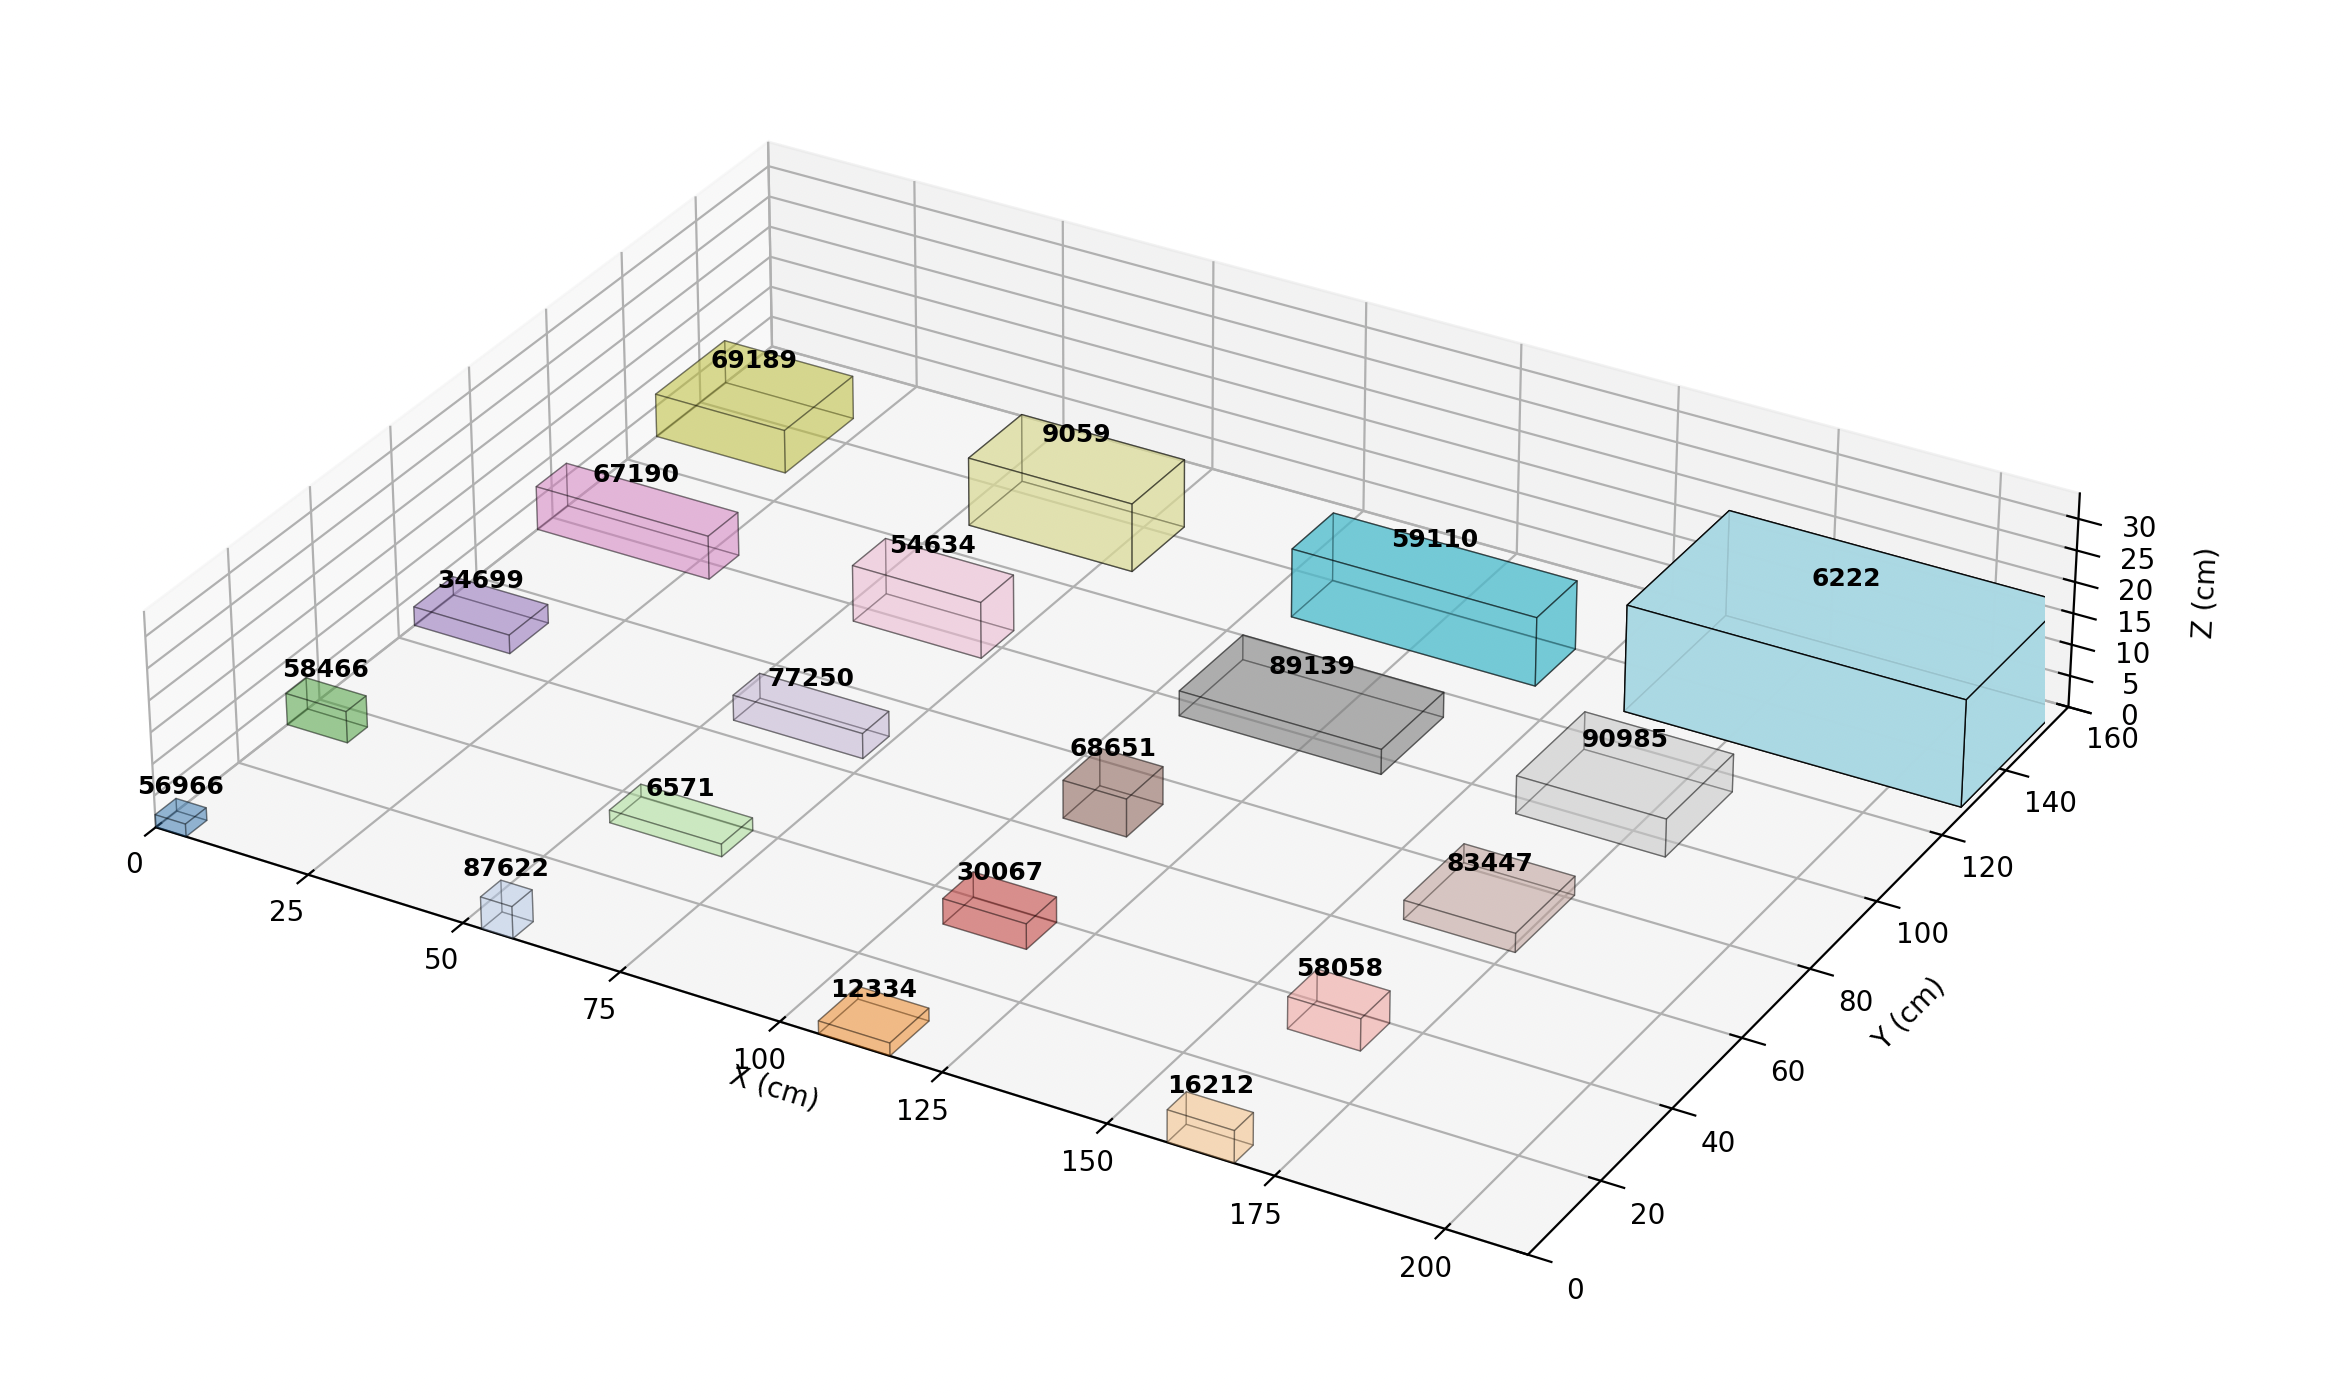
\includegraphics[width=0.85\textwidth]{order.png}
  \caption{Die Eingabetransaktion: alle Produkte mit ihren
           Dimensionen und Gewichten.}
  \label{fig:order}
\end{figure}

%%────────────────────────────────────────────────
\subsubsection{Transaktionstrennung (Abschnitt~\ref{sec:s0})}

Das Transaktionstrennung-MILP zerlegt die Transaktion in
Teiltransaktionen.
Dabei werden die Gewichtskapazit\"at pro Bin, die maximale
Produktanzahl und die Inkompatibilit\"atsbedingungen
(stark unterschiedliche Gewichte) eingehalten.
Das Ergebnis ist eine minimale Anzahl von Teiltransaktionen, die
jeweils einem Karton entsprechen.

Abbildung~\ref{fig:separated} zeigt das Ergebnis: die Produkte sind
in Teiltransaktionen (die Zeilen auf dem Bild) aufgeteilt, sodass keine logistischen oder
physikalischen Beschr\"ankungen verletzt werden.

\begin{figure}[H]
  \centering
  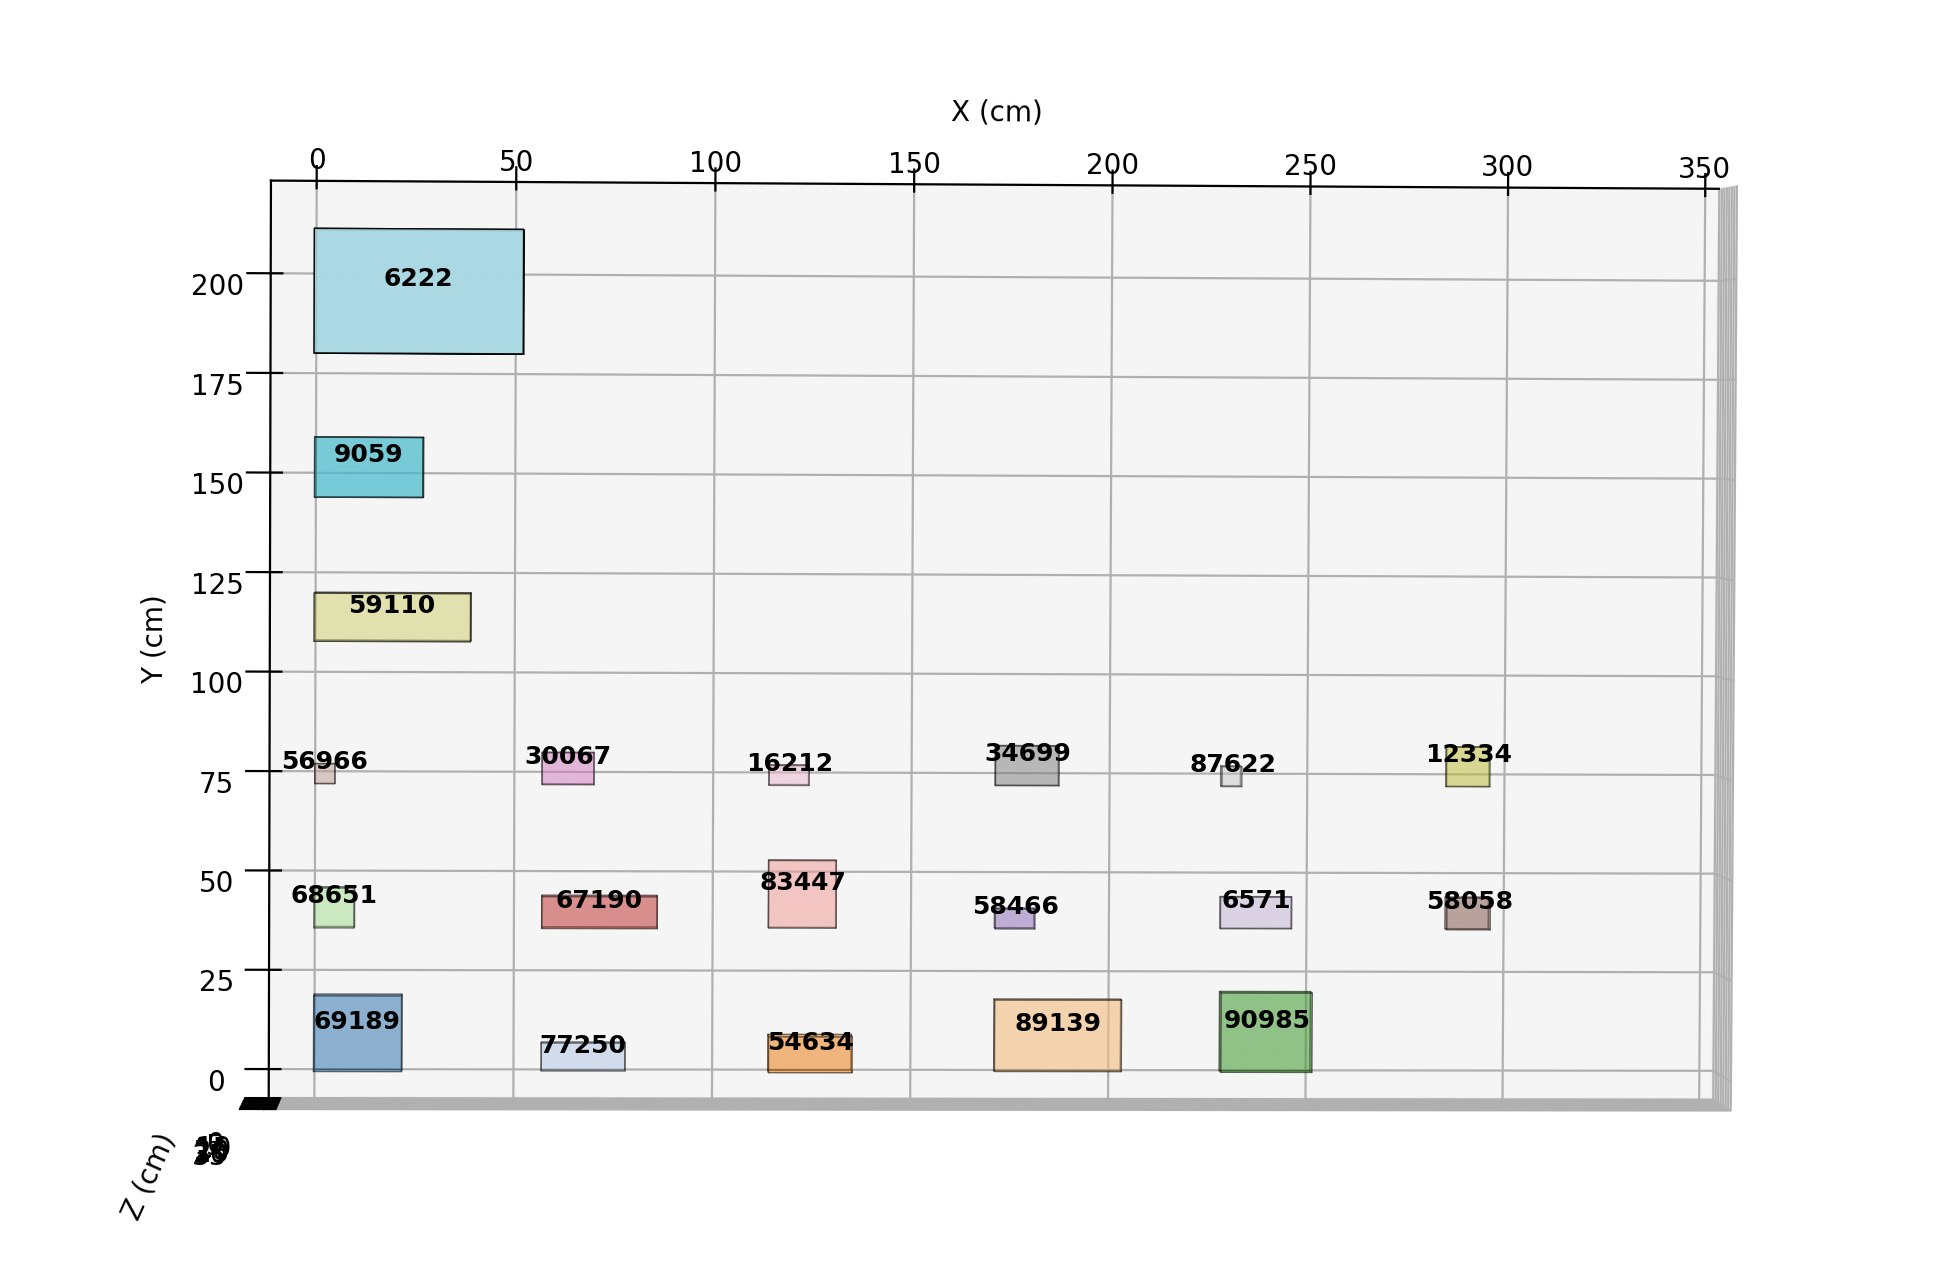
\includegraphics[width=0.85\textwidth]{separated.png}
  \caption{Ergebnis der Transaktionstrennung: die Produkte sind in
           zul\"assige Teiltransaktionen aufgeteilt.}
  \label{fig:separated}
\end{figure}

%%────────────────────────────────────────────────
\subsubsection{Boxauswahl (Abschnitt~\ref{sec:boxauswahl})}
Im Folgenden betrachten wir exemplarisch die 5.~Teiltransaktion
aus Schritt~1 (Transaktionstrennung).
Diese enth\"alt urspr\"unglich 6~Produkte; in der gew\"ahlten Box
werden jedoch nur 5~davon gepackt.
Produkt~83447 konnte nicht untergebracht werden, da es in die
gew\"ahlte Box nicht hineinpasst und die n\"achstgr\"o\ss ere
verf\"ugbare Box die 50\,\%-Freiraumrestriktion verletzen w\"urde.

F\"ur jede Teiltransaktion w\"ahlt das Boxauswahl-MILP einen passenden
Kartontyp aus dem vorgegebenen Sortiment.
Gleichzeitig wird eine geometrisch g\"ultige 3D-Packung erzeugt:
alle Produkte liegen \"uberlappungsfrei im gew\"ahlten Karton, die
Kardinalit\"atsgrenze wird eingehalten, und der Mindestf\"ullgrad
von~$50\%$ ist erf\"ullt.

Abbildung~\ref{fig:box_choosen} zeigt die gew\"ahlten Kartons mit
der initialen, zul\"assigen Packung.
Diese Packung ist geometrisch korrekt, jedoch noch nicht hinsichtlich
physikalischer Stabilit\"at optimiert.

\begin{figure}[H]
  \centering
  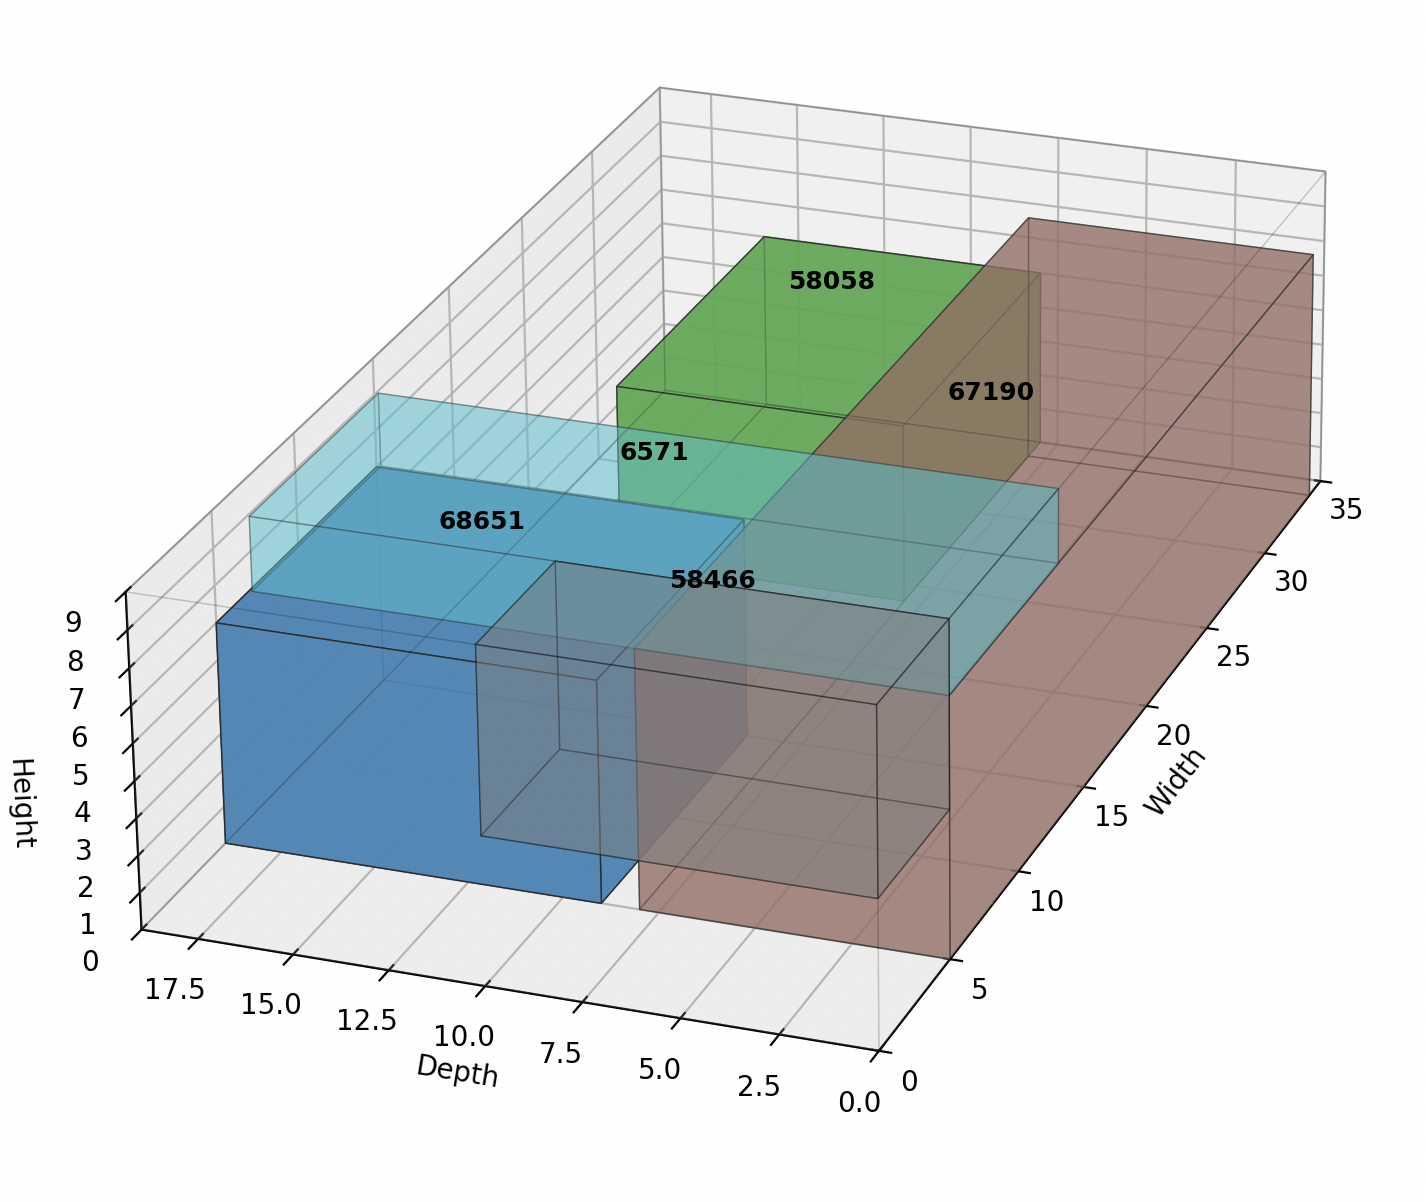
\includegraphics[width=0.85\textwidth]{box_choosen.png}
  \caption{Ergebnis der Boxauswahl: jeder Teiltransaktion ist ein
           Kartontyp zugewiesen, und eine zul\"assige 3D-Packung
           liegt vor.}
  \label{fig:box_choosen}
\end{figure}

%%────────────────────────────────────────────────
\subsubsection{3D-Packqualit\"at (Abschnitt~\ref{sec:s2})}

Das 3D-Packqualit\"at-MIQP nimmt die Ausgabe der Boxauswahl als
Warmstart und optimiert die r\"aumliche Anordnung.

Abbildung~\ref{fig:packing_optimal} zeigt die finale, qualit\"atsoptimierte
Packung.
Im Vergleich zu Abbildung~\ref{fig:box_choosen} sind die Produkte
nun physikalisch sinnvoll angeordnet. Die Packung ist insgesamt stabiler und transportsicherer.

\begin{figure}[H]
  \centering
  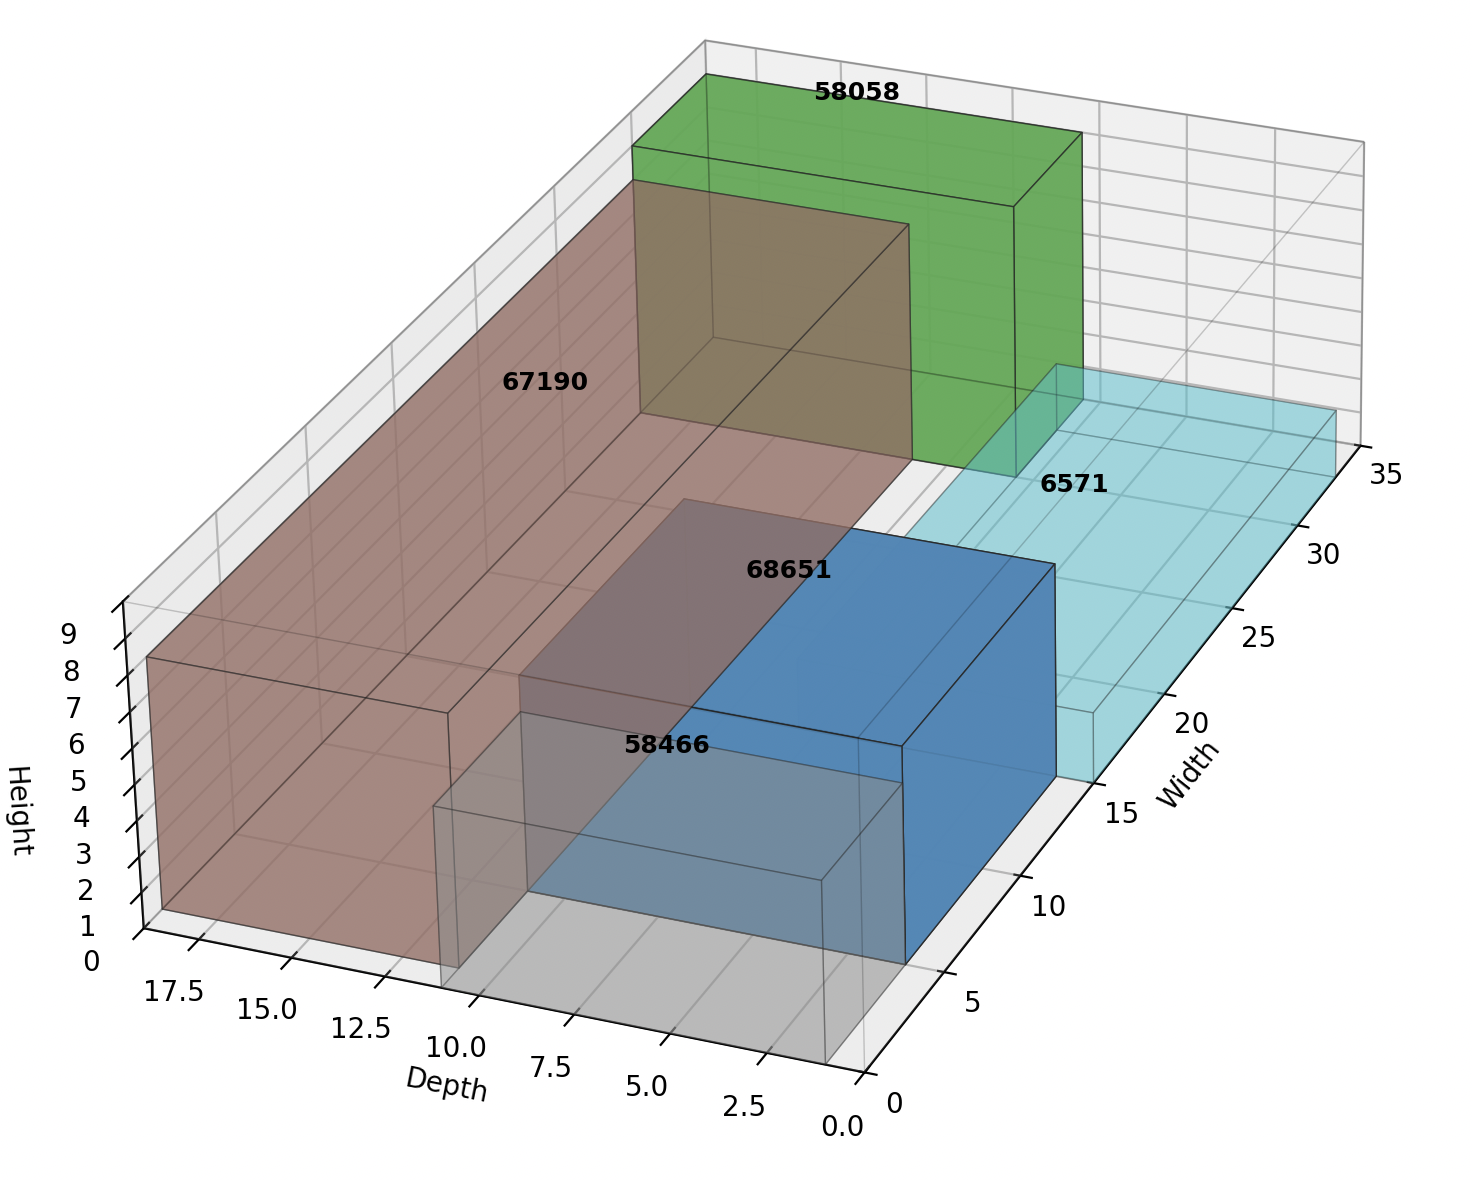
\includegraphics[width=0.85\textwidth]{packing_optimal.png}
  \caption{Finale Packung nach der Qualit\"atsoptimierung:
           physikalisch stabile, transportsichere Anordnung.}
  \label{fig:packing_optimal}
\end{figure}

\begin{table}[H]
\centering
\begin{tabular}{|r|r|r|r|r|}
\hline
ID & flat & pyra & grav & frag \\
\hline
68651 & 0.0 & 0.0 & 0.0 & 0.00 \\
58058 & 15.1 & 0.0 & 0.0 & 0.00 \\
67190 & 0.0 & 0.0 & 0.0 & 0.00 \\
83447 & 0.0 & 0.0 & 0.0 & 0.00 \\
58466 & 0.0 & 0.0 & 0.0 & 0.00 \\
6571 & 0.0 & 0.0 & 0.0 & 0.00 \\
$\Sigma$ & 15.1 & 0.0 & 0.0 & 0.00 \\
\hline
\end{tabular}
\caption{Zerlegter Zielfunktionswert}
\label{tab:objective_terms}
\end{table}

Produkt~58058 ist das einzige mit einem positiven Flachheitswert,
da es nicht auf seiner gr\"o\ss ten Seitenfl\"ache aufliegt.
Die Flachheitsstrafe bestraft genau diese Situation: Wenn ein Produkt
auf einer kleineren Seitenfl\"ache platziert wird, erh\"oht sich der
Zielfunktionswert proportional zum Verh\"altnis zwischen gr\"o\ss ter
und aktueller Auflagefl\"ache.
Alle anderen Produkte liegen bereits auf ihrer maximalen Seitenfl\"ache
und erhalten daher einen Flachheitswert von~$0$.

\subsubsection{Performance}

Alle Konstanten und Gewichte entsprechen den in den vorangehenden
MILP-Formulierungen definierten Werten.

\begin{table}[H]
\centering
\begin{tabular}{|l|l|}
\hline
\textbf{Parameter} & \textbf{Wert} \\
\hline
Solver & Gurobi Optimizer 13.0.0 (build v13.0.0rc1, mac64[arm]) \\
Betriebssystem & Darwin 25.3.0 25D2128 \\
CPU & Apple M2 Pro \\
Threads & 10 physische Kerne, 10 logische Prozessoren (bis zu 10 Threads) \\
\hline
Transaktionstrennung & 0.05\,s CPU-Zeit \\
Boxauswahl & 0.07\,s CPU-Zeit \\
3D-Packqualit\"at (inkl.\ Warmstart) & 0.08\,s CPU-Zeit \\
\hline
\end{tabular}
\caption{Hardware und Laufzeiten f\"ur die 5.~Teiltransaktion.}
\label{tab:performance}
\end{table}

\end{document}
